\documentclass{article}
\usepackage[utf8]{inputenc}
\usepackage{listings}
\usepackage{graphicx}
\graphicspath{ {./images/} {./plots/} }

\title{Computer Graphics: Project}
\author{Bo Kleynen}

\begin{document}

\maketitle

\section{Bounding Volume Hierarchy Construction}
A \textit{bounding volume hierarchy} (BVH) is an acceleration structure in which the objects of the scene are partitioned, in contrast, a k-d tree partitions the space of the scene. The leaves of the BVH contain the geometric objects and the internal nodes store a bounding box of the objects in each of its two sub-trees.

This section compares different heuristics for constructing a BVH in terms of how efficient it is to render a scene. In an ideal case the BVH is a full binary tree for which no bounding boxes overlap on the same level, which means that no 2 sub-trees of a node will ever have to be visited. With these assumptions in mind, the amount of intersection tests required to render a scene can be calculated as:
\begin{equation}
resolution * 2 * \log_{2}{N}
\end{equation}
for N objects in the scene. The multiplication by 2 comes from the fact that at each level 2 bounding boxes have to be intersected.

The experiments in this section use a predetermined set of 10 seeds in order to make sure the scenes are equal for the different heuristics and reduce the impact of randomness in the results. The geometric objects are placed in a unit cube centered around $(0, 0, -1)$, the camera is positioned at the origin with the up-vector point along the positive y-axis. All images are rendered at a resolution of 640 by 640 pixels. The intersection counts shown are for the primary viewing ray only.


\subsection{Uniformly distributed spheres}
To get an initial impression of how the BVH will behave when performing ray intersection queries depending on which heuristic was used to construct it, spheres are uniformly distributed inside the unit cube with a fixed radius R, R is chosen in such a way that the volume of the unit cube that is filled with spheres remains constant.

\begin{figure}[!htb]
    \centering
    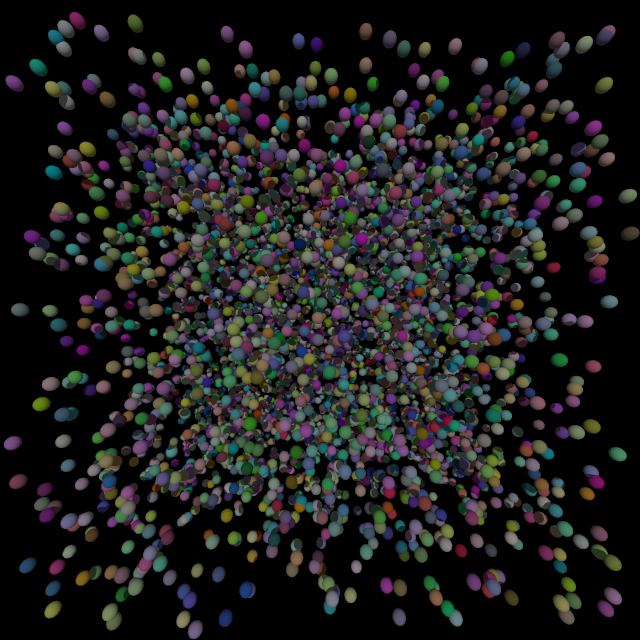
\includegraphics[width=6cm]{renders/equal_spheres_uniform_position.png}
    \caption{5000 equal spheres distributed uniformly over the unit cube}
    \label{fig:equal_spheres_uniform_position}
\end{figure}

Since the scene is uniform, it can be expected that all heuristics will be quite close to each other with the SAH leading slightly because it has a superior stop criteria that is based on an actual cost metric. The stop criteria for object median split and space median split on the other hand depend only on the amount of objects left or the inability to create another partition. Figure \ref{fig:equal_spheres_uniform_position} shows a rendering of this scene.

\begin{figure}[!htb]
    \centering
    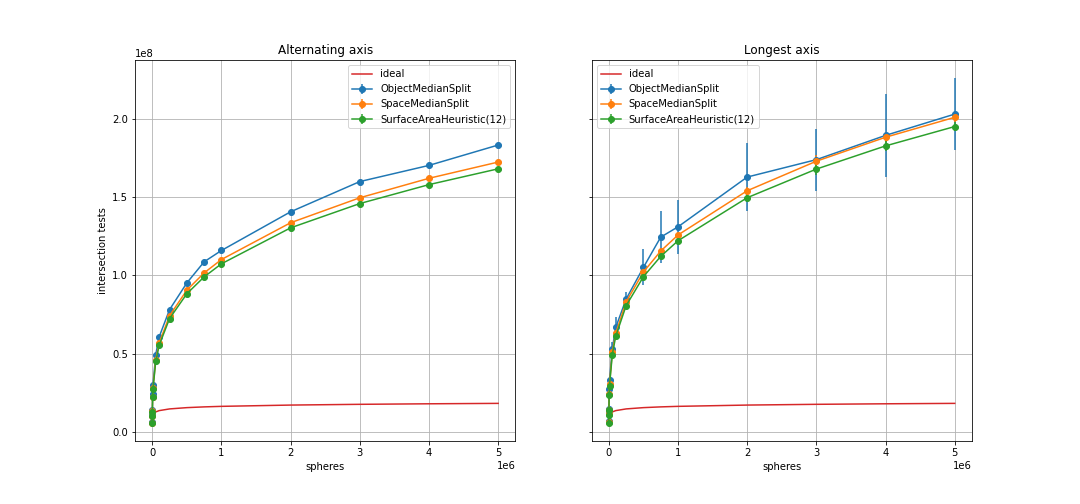
\includegraphics[width=12cm]{plots/splitting_heuristisc_equal_spheres_uniform_position.png}
    \caption{Uniformly distributed spheres with an equal radius}
    \label{fig:splitting_heuristisc_equal_spheres_uniform_position}
\end{figure}

Figure \ref{fig:splitting_heuristisc_equal_spheres_uniform_position} shows the result of this experiment. The SAH did indeed create the best BVH. Another thing worth noting is the high standard deviation when using object median split along the longest axis. The graph also shows clearly that in reality it still takes an order of magnitude more intersection tests to render an image than in the ideal scenario. Remember that we assumed that no bounding boxes overlapped in the ideal case, which is highly unlikely in a realistic scenario.

When comparing this to the amount of intersection tests that would be required without any form of acceleration structure (figure \ref{fig:splitting_heuristisc_equal_spheres_uniform_position_with_naive}), it becomes clear that this difference can be safely ignored in comparison to the speedup gained from using a BVH.

\begin{figure}[!htb]
    \centering
    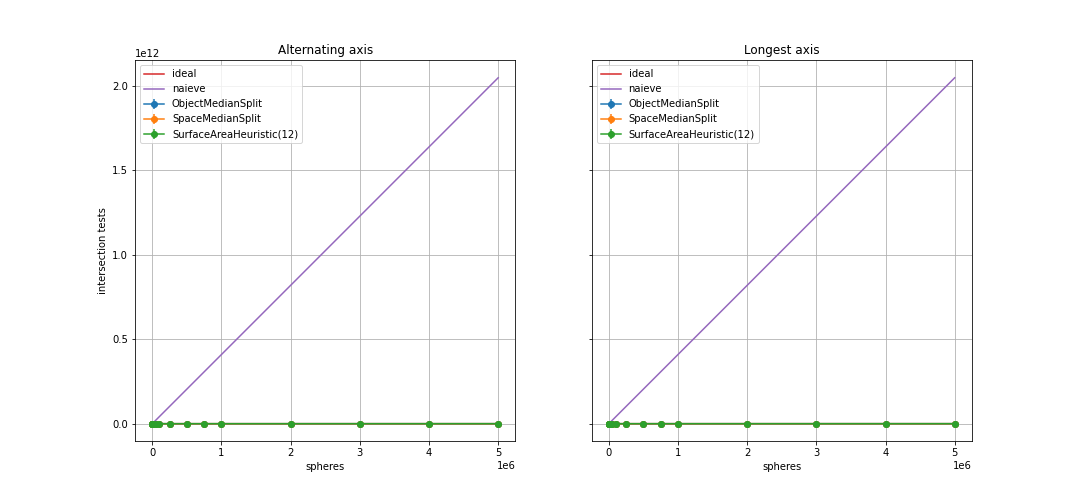
\includegraphics[width=12cm]{plots/splitting_heuristisc_equal_spheres_uniform_position_with_naive.png}
    \caption{Uniformly distributed spheres with an equal radius with naive approach}
    \label{fig:splitting_heuristisc_equal_spheres_uniform_position_with_naive}
\end{figure}

\begin{figure}[!htb]
    \centering
    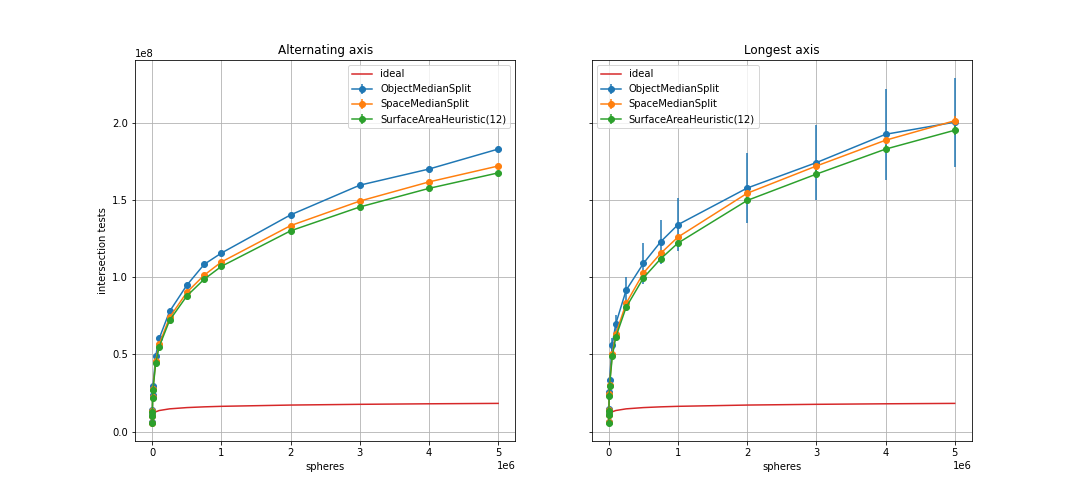
\includegraphics[width=12cm]{plots/splitting_heuristisc_uniform_spheres_uniform_position.png}
    \caption{Uniformly distributed spheres with a uniformly distributed radius}
    \label{fig:splitting_heuristisc_uniform_spheres_uniform_position}
\end{figure}

In the next experiment the radius of each sphere won't be equal, instead it will vary uniformly from a value $R_{min}$ to $5R_{min}$, whilst making sure that the average fill of the unit cube remains constant. The results are shown in figure \ref{fig:splitting_heuristisc_uniform_spheres_uniform_position}. As can be seen in this graph, varying the radius doesn't impact the required amount of intersection tests very much.


\subsection{Non-uniformly distributed spheres}

All experiments in this section are performed with spheres of equal radius as in the first experiment.

The first non-uniform scene uses a normal distribution with $\mu = 0$ and $\sigma = 0.25$ to place spheres along the y and z axis, the position along the x-axis is again uniform. Since most spheres are located around the x-axis, it can be expected that splitting along the longest axis creates better BVHs. From the theory lectures I would expect the heuristics that split along the longest axis construct BVHs that require fewer intersection tests.

\begin{figure}[!htb]
    \centering
    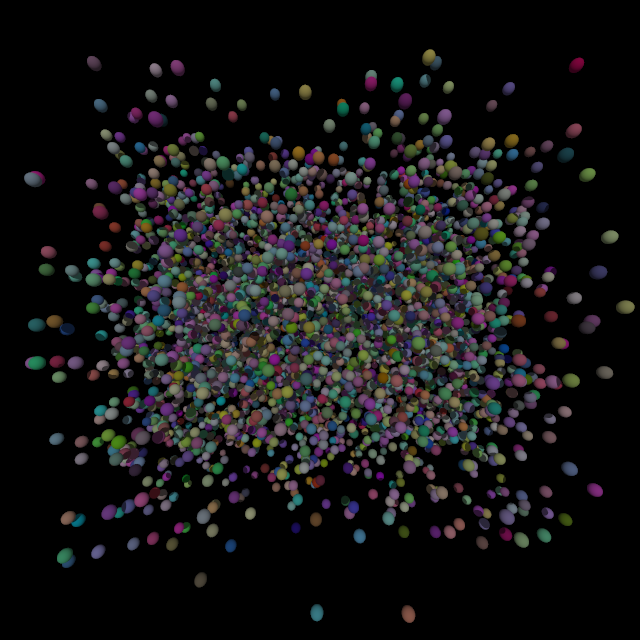
\includegraphics[width=6cm]{renders/equal_spheres_normal_yz.png}
    \caption{5000 spheres with equal radius placed along the y and z axis according to a normal distribution with $\mu = 0$ and $\sigma = 0.25$ and uniformly along the x-axis}
    \label{fig:my_label}
\end{figure}

\begin{figure}[!htb]
    \centering
    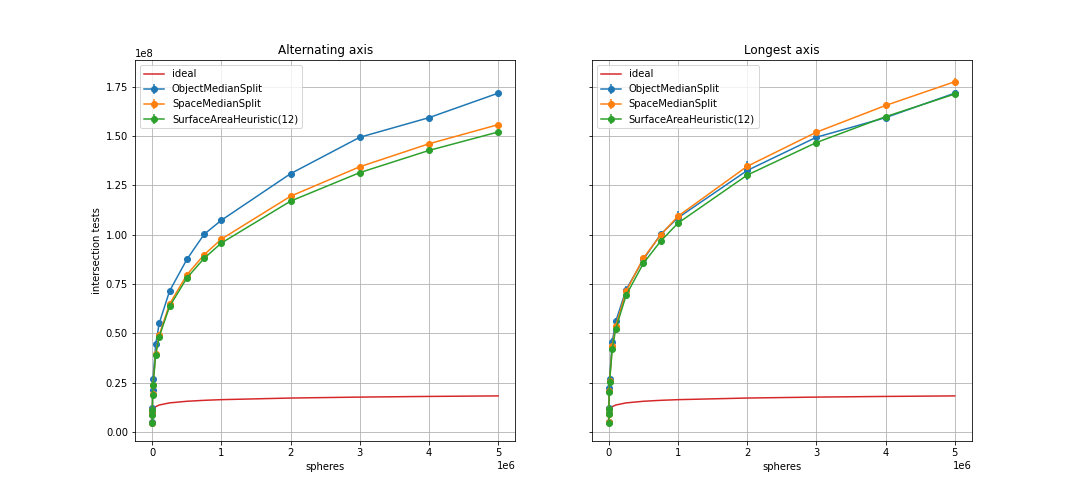
\includegraphics[width=12cm]{plots/splitting_heuristics_equal_spheres_normal_yz.png}
    \caption{Intersection tests for spheres with equal radius that are uniformly distributed along x and normal along y and z with $\mu = 0$ and $\sigma = 0.25$ }
    \label{fig:splitting_heuristics_equal_spheres_normal_yz}
\end{figure}

The experimental results don't seem to support this hypothesis, this could be because there are still a considerable amount of spheres located near the edges of the unit cube to shift the results in favor of alternating. In order to verify this another scene was tested that placed the spheres uniformly, but this time $y \in [-0.2, 0.2]$ and $z \in [-0.2, 0.2]$.

\begin{figure}[!htb]
    \centering
    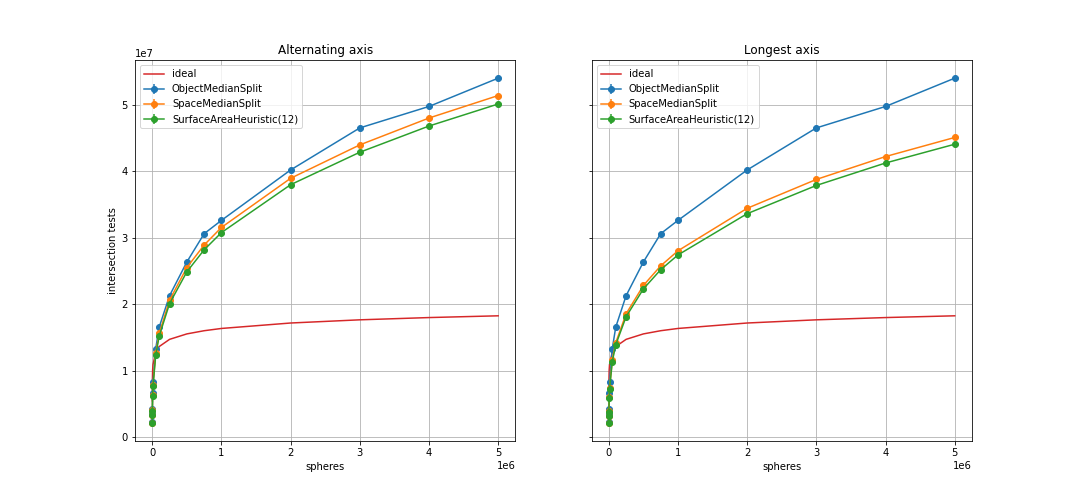
\includegraphics[width=12cm]{plots/splitting_heuristics_equal_spheres_uniform_yz.png}
    \caption{Spheres with equal radius distributed uniformly in a region along the x-axis}
    \label{fig:splitting_heuristics_equal_spheres_uniform_yz}
\end{figure}

Figure \ref{fig:splitting_heuristics_equal_spheres_uniform_yz} confirms this theory. The SAH and space median split along the longest axis are slightly better than the respective heuristic along alternating axis, whilst object median split being equally bad in both scenarios.

The next non-uniform scene places the spheres predominately in the corners and edges of the unit cube by using a beta distribution. This distribution was chosen because it was the only continuous probability distribution that was available on a finite interval and it can be used to generate random values according to a probability density function (PDF) with varying shapes. In this experiment $\alpha = \beta = 0.35$.

Because there are relatively more spheres in the corners of the unit cube I expect the SAH to perform better since it is the only heuristic that can partition the objects in such a way that you get a smaller bounding box with more spheres, which is less likely to be intersected by a ray and a larger bounding box with fewer spheres inside, it will be more likely that this sub tree has to be tested, but testing this sub tree should be less costly.

\begin{figure}[!htb]
    \centering
    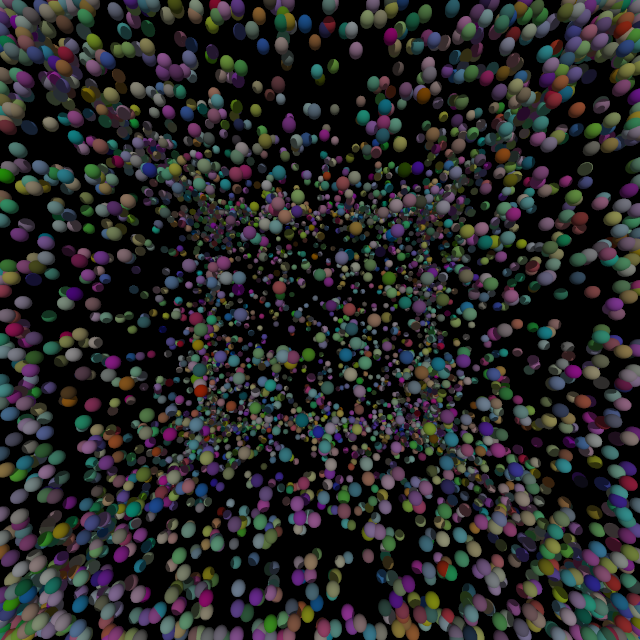
\includegraphics[width=6cm]{renders/equal_spheres_beta_corners.png}
    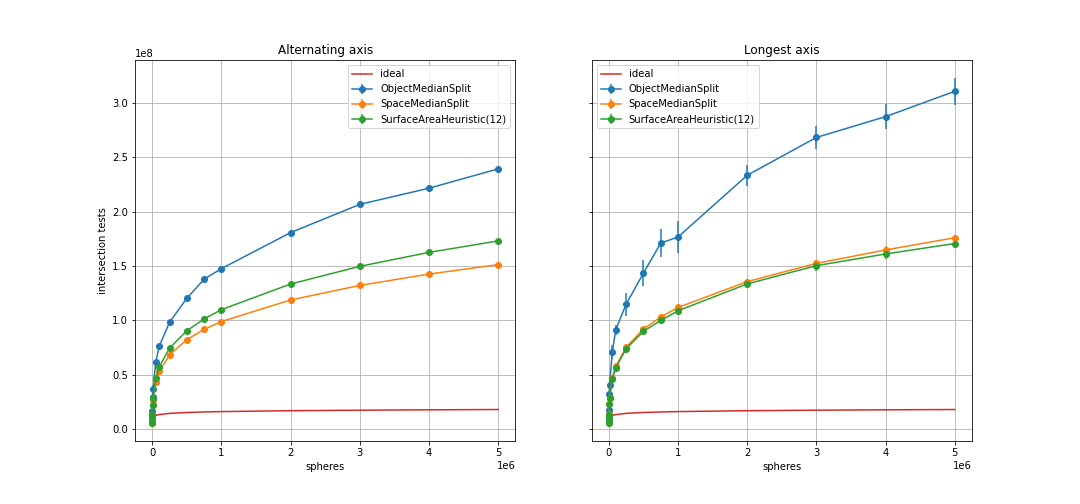
\includegraphics[width=12cm]{plots/splitting_heuristics_equal_spheres_beta_corners.png}
    \caption{Spheres placed according to a beta distribution with $\alpha = \beta = 0.35$}
    \label{fig:splitting_heuristics_equal_spheres_beta_corners}
\end{figure}

\begin{figure}[!htb]
    \centering
    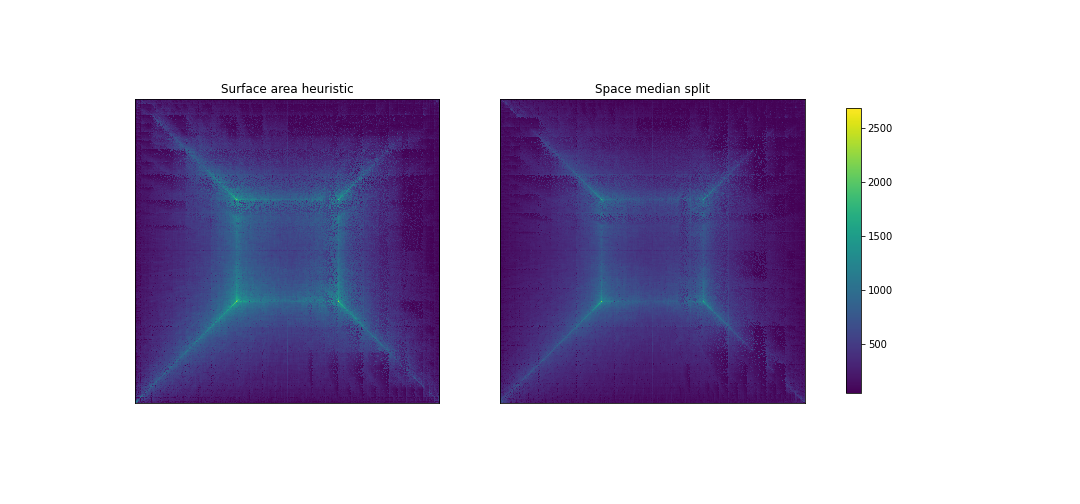
\includegraphics[width=12cm]{plots/splitting_heuristics_equal_spheres_beta_corners_false_color.png}
    \caption{False color images comparing the amount of intersection test required for the SAH and space median split}
    \label{fig:splitting_heuristics_equal_spheres_beta_corners_false_color}
\end{figure}

The results are shown in figure \ref{fig:splitting_heuristics_equal_spheres_beta_corners} and this reveals that the simple space median split with alternating axis performs best for this scene, this is a result for which I don't have an explanation at the time of writing this report. Figure \ref{fig:splitting_heuristics_equal_spheres_beta_corners_false_color} shows the amount of intersection tests required to render each pixel, it shows clearly that the same regions are the most costly. The BVH constructed using the SAH just requires more intersections to render these regions.

\subsection{Conclusion}

From these experiments it can be concluded that axis selection doesn't matter that much unless there is a direction along which the distribution of objects is significantly longer.

The SAH is the constructs the best BVHs in most scenarios, however I would have expected it to be more significantly better than space median split since it is a widely used heuristic.

\section{Instancing}

\subsection{Rendering Performance}

\begin{figure}[!htb]
    \centering
    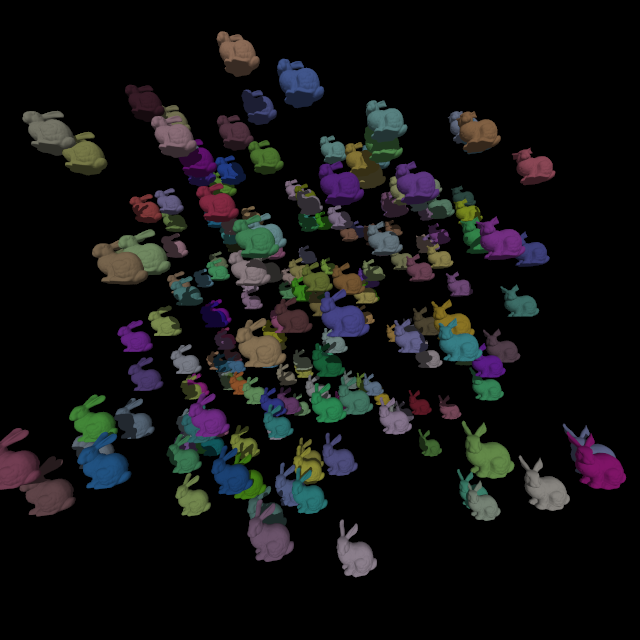
\includegraphics[width=6cm]{renders/200_bunnies.png}
    \caption{200 Stanford bunnies uniformly distributed over a unit cube}
    \label{fig:200_bunnies}
\end{figure}

\begin{figure}[!htb]
    \centering
    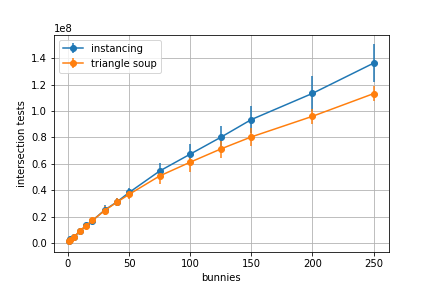
\includegraphics[width=12cm]{plots/instancing_intersection_tests.png}
    \caption{Intersection tests for uniformly distributed bunnies}
    \label{fig:instancing_intersection_tests}
\end{figure}

When instancing is used the mesh data structures have their own acceleration structure that is separate from the one constructed by the world. For the creation of this world BVH only the bounding box of the entire mesh is taken into consideration. This hierarchy of BVHs is called a multi-level BVH.

Because the different parts of a multi-level BVH are created without knowledge of the rest of the world the final BVH will be less optimal than what would be possible if a singel BVH was created from a triangle soup. This last approach is better suited to take into account overlapping instances.

In this experiment bunnies were placed uniformly in a unit cube as in the previous section, this time however they were always the same size instead of aiming for a constant filled volume as the volume of a bunny is quite hard to determine. The scaling factor of the bunnies was chosen in such a way that not too many bunnies overlapped, even at higher amounts of bunnies. Figure \ref{fig:200_bunnies} shows a rendering of this scenario for 200 bunnies.

The experiment shows that for larger amounts of bunnies instancing requires slightly more intersection tests to render the scene (figure \ref{fig:instancing_intersection_tests}). While performing the experiments I did notice however it took increasingly more time to construct the BVH when not using instancing. I did not perform a thorough study of this effect, but my initial impression was that in total instancing had better performance for the tested scenes

\subsection{Memory usage}

On of the greatest benefits of instancing is that it uses less memory, this section investigates this aspect of instancing. The experiment uses jemalloc as its heap allocator instead of the default macOS one because it provides utilities to measure the allocated heap memory. In order to measure the amount of heap memory allocated for the world data structure, the total heap memory of the was measured before and after its creation, the difference is then the amount of memory that had to be allocated for the world data structure. The world contains everything necessary to render the scene (triangles, materials, transformation matrices, lights, ...).

Since instancing requires very little additional data in order to add another instance, just the transformation matrix and a pointer to the original mesh data structure, the allocated heap memory should be approximately constant. When creating a triangle soup on the other hand, the triangles have to be duplicated for every new instance so the amount of memory required should increase linearly with the amount of bunnies.

The results of the experiment that can be found in figure \ref{fig:instancing_heap_memory} and do suggest that this hypothesis is correct.

\begin{figure}[!htb]
    \centering
    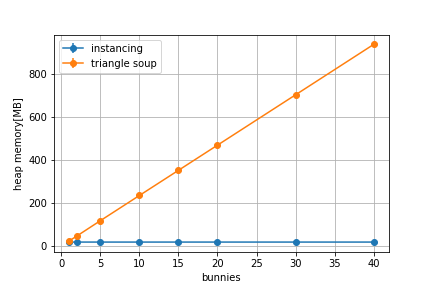
\includegraphics[width=12cm]{plots/instancing_heap_memory.png}
    \caption{Heap memory allocated for the world data structure}
    \label{fig:instancing_heap_memory}
\end{figure}

\subsection{Implementation}

It should be taken into account that the original implementation of the BVH already used instancing. Another advantage of instancing is that it was easier to implement and use when building scenes. The use of instancing isn't limited to triangle meshes, it can also be used to reuse certain parts of a scene, which makes it easier to compose complex scenes out of smaller components.

To go from an implementation that used the same data structures for instancing and more generally any transformed object to an experiment that had every triangle instanced in the world proved to be non-trivial. There are two possible approaches to this problem. Either manually duplicate all the necessary data structures (this approach was used for the experiments as it didn't involve changing any of the rendering code) or introduce a separate translation step, which has the major drawback that every data structure used in creating the scene graph has to be cloneable (= implement the Clone trait in Rust), which wasn't the case in my implementation as it was build with instancing from the start.

\subsection{Conclusion}

Given the many benefits of instancing, it is a sane default and pouring everything into a triangle soup should only be considered when there is sufficient evidence that the reduction in amount of intersection tests will offset the increase BVH construction time.

\section{Textures}

I still had to provide a picture of an image with a texture:
\begin{figure}[hb]
    \centering
    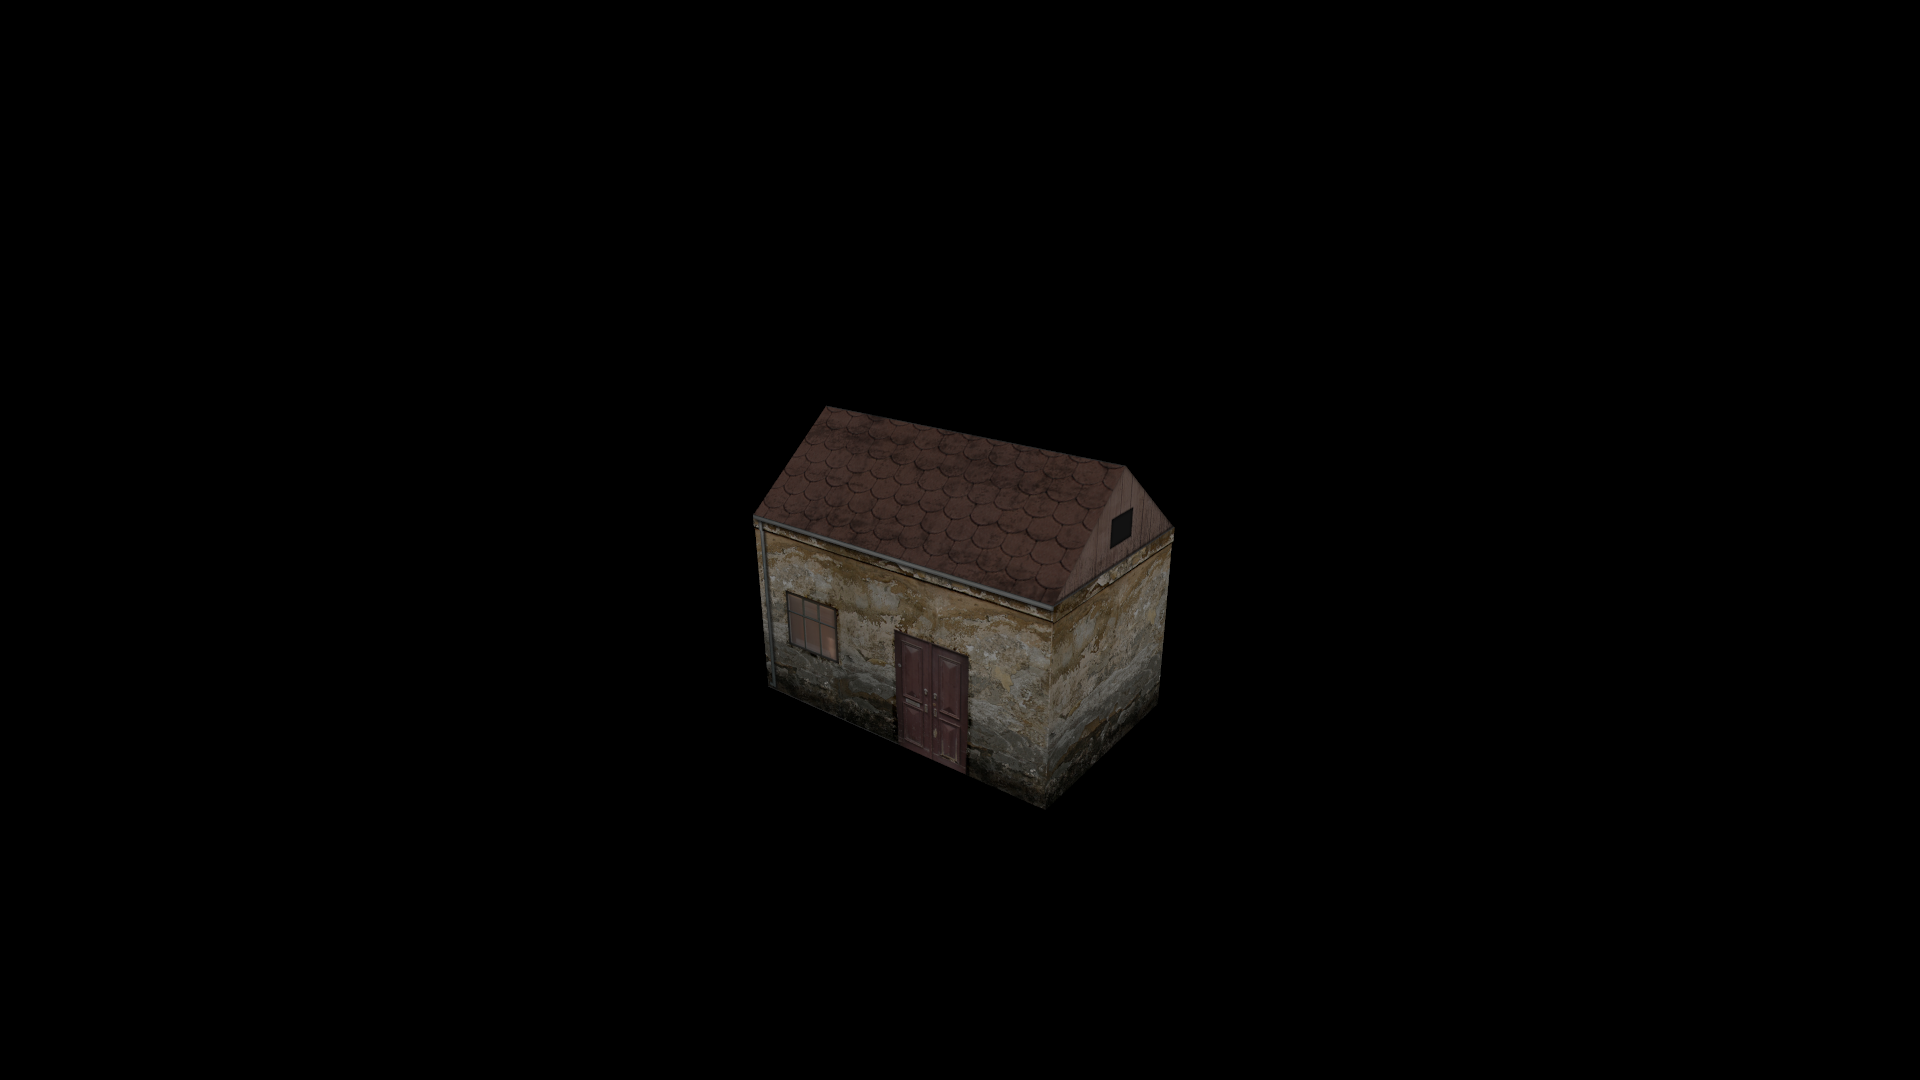
\includegraphics[width=12cm]{renders/house.png}
    \caption{A house with texture}
\end{figure}

% \section{Reflection on the usage of rust}

% Please note that this section is an opinion piece and thus highly subjective.

% As the title of this section might suggest I implemented my ray tracer entirely in rust. The fact that I was allowed to do this in rust was actually one of the main reasons I took this class (pretty pictures of spheres was also a major reason). Rust has several features that makes it a better choice for this kind of applications.

% It has the same performance characteristics as C++, the language that is used to implement most production ray tracers and most ray tracing text books. It compiles to native machine instructions with virtually no run time, compared to Java which is only compiled to java byte code which is then interpreted by the JVM, a program that is notoriously memory hungry.

% You might wonder why not just use C++ like everyone else, the answer to this question can be given with one word: safety. Rust uses its type system to guarantee that all memory access is valid and that you wont encounter any data races, that is of course if you refrain from using the unsafe keyword, which lets you dereference arbitrary pointers. I must admit that I used unsafe in a couple of places to gain some performance, but these usages should be perfectly safe, and some of them avoidable in the future when "Generic Associated Types" will be implemented.

% This points towards maybe the biggest drawback of Rust, it is a relatively young language (it only hit 1.0 6 years ago) and whilst this didn't prove to be a big problem for me during this project, I could easily find the libraries I needed, it might be off putting for people to use it for production ray tracers. On the notion of libraries, Cargo is a fantastic build system.

% % TODO

% I would certainly advise future students that know some basic rust to consider it for this project, depending on your knowledge of rust you might have to put in a bit of extra work to research certain features. For me this would also have been the case for Java however and probably even more so because outside of the courses where it is mandatory to use it, I don't program in Java and I sincerely hope I will never have to program in Java again.

\end{document}
